\documentclass[tikz]{standalone}
\usepackage{pgfplots}
\pgfplotsset{compat=1.15}
\usepackage{mathrsfs}
\usetikzlibrary{arrows,calc}
\usepackage{tkz-euclide}
\pagestyle{empty}

\definecolor{AngleClr}{rgb}{0,0.39215686274509803,0}
\definecolor{ShapeClr}{rgb}{0.6,0.2,0}
\definecolor{BlueClr}{RGB}{13,93,184}

\begin{document}

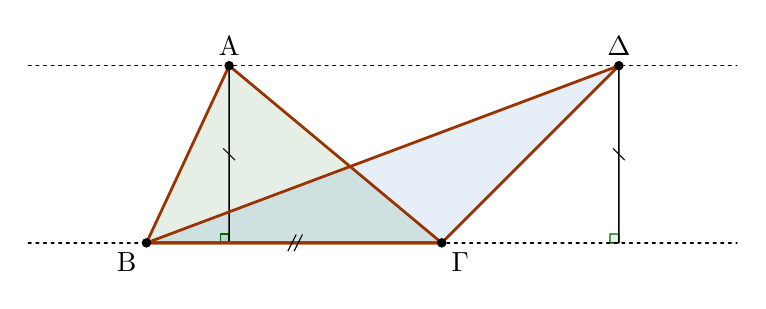
\begin{tikzpicture}[scale=.75]
\tkzSetUpLine[line width=1pt,color=black]
\tkzSetUpPoint[fill=black]

\tkzDefPoints{0/0/B,1.4/3/A,5/0/C,8/3/D}

\tkzDefPoints{-2/3/L1,10/3/R1}
\tkzDefPoints{-2/0/L2,10/0/R2}

\tkzDefPointBy[projection=onto B--C](A)\tkzGetPoint{AA}
\tkzDefPointBy[projection=onto B--C](D)\tkzGetPoint{DD}
\tkzMarkRightAngles[line width=0.5pt, size=.15,color=AngleClr,fill=AngleClr,fill opacity=0.1](A,AA,B D,DD,C)


\tkzFillPolygon[fill=AngleClr,fill opacity=0.1](A,B,C)
\tkzFillPolygon[fill=BlueClr,fill opacity=0.1](B,C,D)


\tkzDrawSegments[line width=0.5pt,color=black,dashed,dash pattern=on 1pt off 1.75pt](L1,R1 L2,R2)
\tkzDrawSegments[line width=0.5pt,color=black](A,AA D,DD)
\tkzDrawPolygon[color=ShapeClr](A,B,C)
\tkzDrawPolygon[color=ShapeClr](B,C,D)

\tkzDrawPoints[size=3](A,B,C,D)


\tkzLabelPoint[above](A){$\rm A$}
\tkzLabelPoint[below left](B){$\rm B$}
\tkzLabelPoint[below right](C){$\rm \Gamma$}
\tkzLabelPoint[above](D){$\rm \Delta$}

\tkzMarkSegments[mark=s||,size=3](B,C)
\tkzMarkSegments[mark=s|,size=3](A,AA D,DD)

\end{tikzpicture}

\end{document}
